\let\negmedspace\undefined
\let\negthickspace\undefined
\documentclass[journal]{IEEEtran}
\usepackage[a5paper, margin=10mm, onecolumn]{geometry}
%\usepackage{lmodern} % Ensure lmodern is loaded for pdflatex
\usepackage{tfrupee} % Include tfrupee package

\setlength{\headheight}{1cm} % Set the height of the header box
\setlength{\headsep}{0mm}     % Set the distance between the header box and the top of the text

\usepackage{gvv-book}
\usepackage{gvv}
\usepackage{cite}
\usepackage{amsmath,amssymb,amsfonts,amsthm}
\usepackage{algorithmic}
\usepackage{graphicx}
\usepackage{textcomp}
\usepackage{xcolor}
\usepackage{txfonts}
\usepackage{listings}
\usepackage{enumitem}
\usepackage{mathtools}
\usepackage{gensymb}
\usepackage{comment}
\usepackage[breaklinks=true]{hyperref}
\usepackage{tkz-euclide} 
\usepackage{listings}
% \usepackage{gvv}                                        
\def\inputGnumericTable{}                                 
\usepackage[latin1]{inputenc}                                
\usepackage{color}                                            
\usepackage{array}                                            
\usepackage{longtable}                                       
\usepackage{calc}                                             
\usepackage{multirow}                                         
\usepackage{hhline}                                           
\usepackage{ifthen}                                           
\usepackage{lscape}
\usepackage{circuitikz}
\tikzstyle{block} = [rectangle, draw, fill=blue!20, 
    text width=4em, text centered, rounded corners, minimum height=3em]
\tikzstyle{sum} = [draw, fill=blue!10, circle, minimum size=1cm, node distance=1.5cm]
\tikzstyle{input} = [coordinate]
\tikzstyle{output} = [coordinate]

\begin{document}

\bibliographystyle{IEEEtran}
\vspace{3cm}

\title{2.5.5}
\author{EE25BTECH11051 - Shreyas Goud Burra}
\maketitle
% \newpage
% \bigskip
{\let\newpage\relax\maketitle}

\renewcommand{\thefigure}{\theenumi}
\renewcommand{\thetable}{\theenumi}
\setlength{\intextsep}{10pt} % Space between text and floats


\numberwithin{equation}{enumi}
\numberwithin{figure}{enumi}
\renewcommand{\thetable}{\theenumi}

\textbf{Question}
Write the projection of the vector ($\vec{b} + \vec{c}$) on the vector $\vec{a}$, where $\vec{a} = 2\hat{i}-2\hat{j}+\hat{k}$, $\vec{b} = \hat{i}+2\hat{j}-2\hat{k}$, and $\vec{c} = 2\hat{i}-\hat{j}+4\hat{k}$.\\

\solution\\

Let us find the solution theoretically first and then verify it computationally.

Let the vectors be represented as \textbf{A}, \textbf{B}, and \textbf{C} respectively. Given by

\begin{align}
    \textbf{A} = \myvec{2 \\ -2 \\ 1}, \textbf{B} = \myvec{1 \\ 2\\ -2}, \textbf{C} = \myvec{2\\-1\\4}
    \label{0.1}
\end{align}

Mathematically, the projection of the vector \textbf{B}+\textbf{C} on the vector \textbf{A} is given by some vector \textbf{D},

\begin{align}
    \textbf{D} = k\textbf{A}\text{, such that } ((\textbf{B}+\textbf{C})-\textbf{D})^\text{T}\textbf{D}=0
    \label{0.2}
\end{align}

yielding,

\begin{align}
    ((\textbf{B}+\textbf{C})-k\textbf{A})^\text{T}\textbf{A}=0
    \label{0.3}
\end{align}

or,


\begin{align}
    k=\frac{(\textbf{B}+\textbf{C})^\text{T}\textbf{A}}{\norm{\textbf{A}}^2} \implies \textbf{D} = \frac{(\textbf{B}+\textbf{C})^\text{T}\textbf{A}}{\norm{\textbf{A}}^2}\textbf{A}
    \label{0.4}
\end{align}


On substituting the values,

\begin{align}
    \textbf{D} = \frac{\brak{\myvec{1\\2\\-2}+\myvec{2\\-1\\4}}^\text{T}\myvec{2\\-2\\1}}{\norm{\myvec{2\\-2\\1}}^2}\myvec{2\\-2\\1}
    \label{0.5}
\end{align}

\newpage

On calculation, this gives us,

\begin{align}
    \textbf{D} = \myvec{4/3\\-4/3\\2/3}
    \label{0.6}
\end{align}

We get the same result by plotting a graph for the following.
\begin{figure}[H]
    \centering
    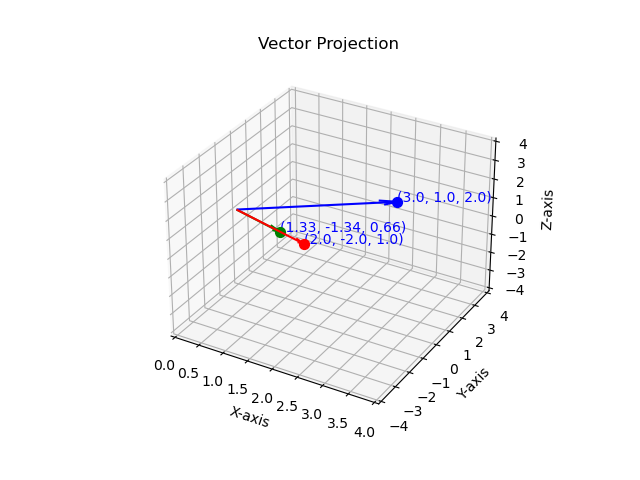
\includegraphics[width=0.8\columnwidth]{figs/fig1.png}
    \caption{3D Plot}
    \label{3D Plot}
\end{figure}





\end{document}
